\chapter{Progettazione del sistema}

\section{Introduzione all'UML}
In questo capitolo verrà trattata la progettazione e la modellazione del sistema attraverso uno strumento molto diffuso nello sviluppo delle applicazioni: UML. 


In ingegneria del software, UML è un linguaggio di modellazione e di specifica basato sul paradigma orientato agli oggetti. Il linguaggio nacque con l'intento di unificare approcci precedenti, raccogliendo le migliori prassi nel settore e definendo così uno standard industriale unificato.

\section{Architettura di riferimento}

Nell'ingegneria del software, il termine architettura multi-tier o architettura multi-strato indica un'architettura software in cui le varie funzionalità del software sono logicamente separate ovvero suddivise su più strati o livelli software differenti in comunicazione tra loro.

Ciascuno strato è in comunicazione diretta con quelli adiacenti ovvero richiede ed offre servizi allo strato adiacente in maniera concettualmente simile a quanto accade con le architetture di rete a strati.

Nello specifico, in questa applicazione è stato usato il pattern MVC, ovvero il \textit{Model-View-Controller} che, in informatica, è un pattern architetturale molto diffuso nello sviluppo di sistemi software, in particolare nell'ambito della programmazione orientata agli oggetti, in grado di separare la logica di presentazione dei dati dalla logica di business.

Questo pattern si posiziona nel livello logico o di business e di presentazione in una architettura multi-tier.

Il componente centrale del MVC, il modello, cattura il comportamento dell'applicazione in termini di dominio del problema, indipendentemente dall'interfaccia utente. Il modello gestisce direttamente i dati, la logica e le regole dell'applicazione. Una vista può essere una qualsiasi rappresentazione in output di informazioni, come un grafico o un diagramma. Sono possibili viste multiple delle stesse informazioni, come ad esempio un grafico a barre per la gestione e la vista tabellare per l'amministrazione. La terza parte, il controller, accetta l'input e lo converte in comandi per il modello e/o la vista.

\begin{figure}[H]
	\centering
	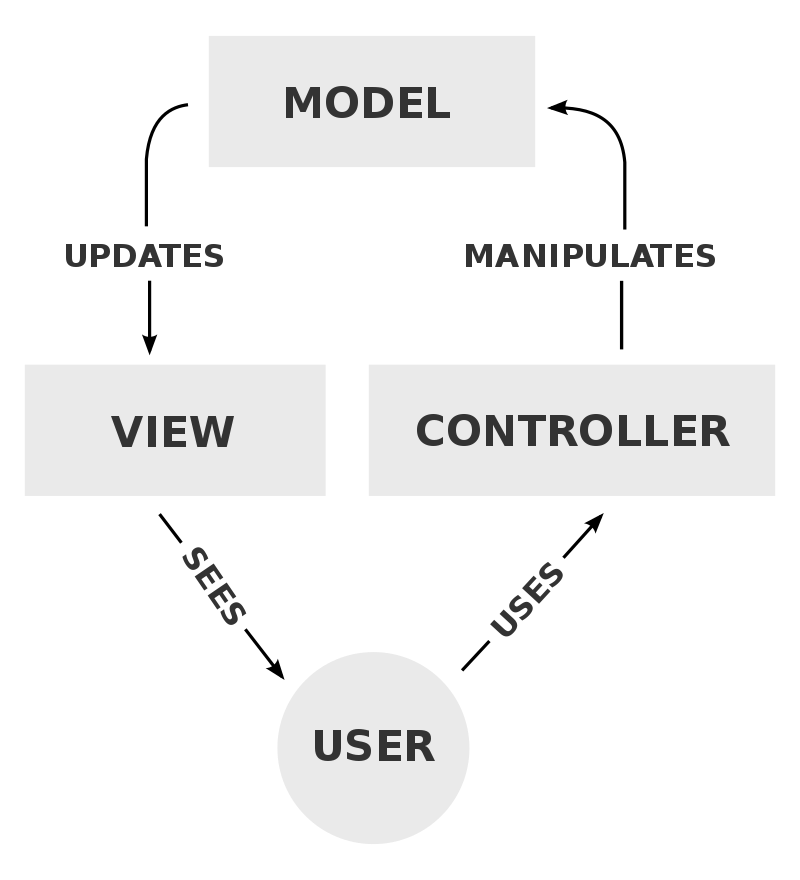
\includegraphics[width=0.5\textwidth]{./media/MVC.png}
	\caption{Architettura MVC schematizzata}
\end{figure}

\section{Diagramma delle classi}
Il diagramma delle classi consente di descrivere le entità del progetto, rappresentandoli con le loro caratteristiche e mettendole in relazione tra loro.

In questa sezione viene presentato il diagramma delle classi di Inline con i relativi requisiti e le specifiche necessarie alla gestione della classe Utente e delle varie classi ad essa connesse.		
Degli utenti interessa:
\begin{itemize}
	\item Id
	\item Username
	\item Email
	\item Password
	\item Numero delle room a cui ha partecipato
	\item Il suo rating
	\item Data creazione
	\item Ultima modifica
\end{itemize}
In oltre, qualsiasi utente può in qualsiasi momento eliminare il proprio account, creare una room e inviare un messaggio.

Delle rooms interessa:
\begin{itemize}
	\item Id
	\item Name
	\item Descrizione
	\item Tipo di coda
	\item Numero massimo partecipanti
	\item Indirizzo
	\item Longitudine
	\item Latitudine
	\item Se è privata
	\item Data creazione
	\item Data terminazione
	\item Id del creatore
	\item Id dell evento
\end{itemize}

Dei messaggi interessa:
\begin{itemize}
	\item Id
	\item Id della room
	\item Id dell'utente
	\item Tipo del destinatario
	\item Id del destinatario
	\item Notification id
	\item Campi per denotare se il messaggio è stato letto, cancellato
	\item Campo per la creazione del messaggio
	\item Campo per la modifica del messaggio
\end{itemize}
\begin{figure}[H]
	\centering
	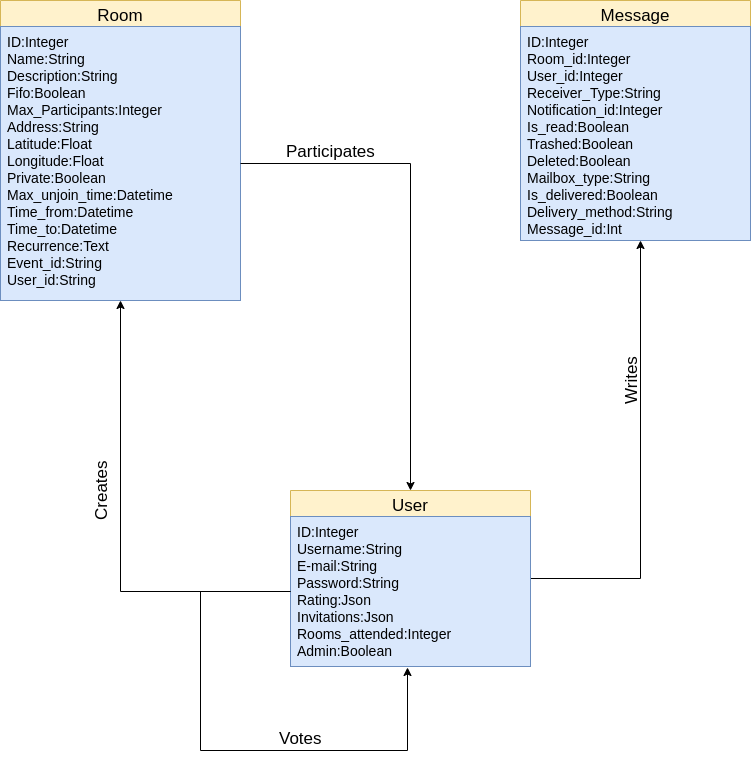
\includegraphics[width=\textwidth]{./media/UML.png}
	\caption{Diagramma UML delle classi}
\end{figure}

Adesso definiremo due operazioni: La delete per l'user e per il messaggio.

\begin{lstlisting}
	InizioSpecificaOperazioneClasse User
		Delete(Id:Integer): User
			Pre:Nessuno
			Post:Utente cancellato
	Fine specifica
\end{lstlisting}
\\
\begin{lstlisting}
	InizioSpecificaOperazioneClasse Message
		Delete(Id:Integer): Message
			Pre:Nessuno
			Post:Messaggio cancellato
	Fine specifica
\end{lstlisting}

\section{Diagramma degli stati}
Il diagramma degli stati è un diagramma previso dall'UML per descrivere il comportamente di classi, mostrando gli stati che sono assunti dall'entità in risposta ad eventi.
Presentiamo il diagramma degli utenti di Inline: Un utente si trova inizialmente in uno stato \textit{Visitatore}. Se un utente effettua il \textit{Signup} diventa registrato. Se l'utente ha effettuato il \textit{Signin}, può mandare un evento \textit{Logout} ed uscire dal sito rimanendo un utente registrato. Se l'utente registrato non ha effettuato l'accesso, può mandare un evento \textit{Signin} ed accedere al sito rimanendo utente registrato. Un utente può passare da uno stato di \textit{Registrato} a \textit{Ospite} in seguto ad un'operazione di delete.

\begin{figure}[H]
	\centering
	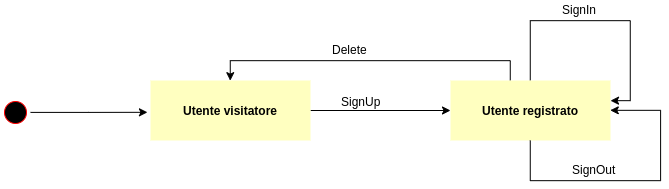
\includegraphics[width=\textwidth]{./media/DiagrammaStati.png}
	\caption{Diagramma degli stati}
\end{figure}

\begin{lstlisting}
	InizioSpecificaStatiClasse User
	Stato: {Visitatore, Registrato}
	Variabili di stato ausiliarie:
		UtenteRegistrato = User
		UtenteLog = User
	Stato Iniziale:
		statoCorrente = Ospite
		utenteRegistrato = Nil
		utenteLog = Nil
	Fine specifica

	InizioSpecificaTransazioni User
		Transazione Ospite -> Registrato (SignUp)
			Evento: Signup
			Condizione: Nessuna
			Azione: 
				Pre: Nil
				Post: UtenteRegistrato = This
		
		Transazione Registrato -> Registrato (SignIn)
			Evento: Sign in
			Condizione: UtenteLog = Nil
			Azione:
				Pre: Nil
				Post: UtenteLog = This
		
		Transazione Registrato -> Registrato (SignOut)
			Evento: SignOut
			Condizione: UtenteLog = This
			Azione:
				Pre: Nil
				Post: UtenteLog = Nil
		
		Transazione Registrato -> Visitatore (Delete)
			Evento: Delete
			Condizione: Nessuna
			Azione:
				Pre: Nil
				Post: UtenteRegistrato = Nil
	FineSpecifica	
\end{lstlisting}

\section{Diagramma delle attività}
